% !TEX TS-program = pdflatex
% !TEX encoding = UTF-8 Unicode

% This is a simple template for a LaTeX document using the "article" class.
% See "book", "report", "letter" for other types of document.

\documentclass[11pt]{article} % use larger type; default would be 10pt

\usepackage[utf8]{inputenc} % set input encoding (not needed with XeLaTeX)

%%% PAGE DIMENSIONS
\usepackage{geometry} % to change the page dimensions
\geometry{a4paper} % or letterpaper (US) or a5paper or....

\usepackage{graphicx} % support the \includegraphics command and options

\usepackage{amssymb}
\usepackage{amsmath}
%%% PACKAGES
\usepackage{booktabs} % for much better looking tables
\usepackage{array} % for better arrays (eg matrices) in maths
\usepackage{paralist} % very flexible & customisable lists (eg. enumerate/itemize, etc.)
\usepackage{verbatim} % adds environment for commenting out blocks of text & for better verbatim
\usepackage{subfig} % make it possible to include more than one captioned figure/table in a single float
% These packages are all incorporated in the memoir class to one degree or another...

%%% HEADERS & FOOTERS
\usepackage{fancyhdr} % This should be set AFTER setting up the page geometry
\pagestyle{fancy} % options: empty , plain , fancy
\renewcommand{\headrulewidth}{0pt} % customise the layout...
\lhead{}\chead{}\rhead{}
\lfoot{}\cfoot{\thepage}\rfoot{}

%%% SECTION TITLE APPEARANCE
\usepackage{sectsty}
\allsectionsfont{\sffamily\mdseries\upshape} % (See the fntguide.pdf for font help)
% (This matches ConTeXt defaults)

%%% ToC (table of contents) APPEARANCE
\usepackage[nottoc,notlof,notlot]{tocbibind} % Put the bibliography in the ToC
\usepackage[titles,subfigure]{tocloft} % Alter the style of the Table of Contents
\renewcommand{\cftsecfont}{\rmfamily\mdseries\upshape}
\renewcommand{\cftsecpagefont}{\rmfamily\mdseries\upshape} % No bold!

\usepackage{amsmath}
\usepackage{graphicx}
\graphicspath{ {./pings/} }
\DeclareMathOperator*{\argmax}{arg\,max}
\DeclareMathOperator*{\argmin}{arg\,min}

\newcount\colveccount
\newcommand*\colvec[1]{
        \global\colveccount#1
        \begin{pmatrix}
        \colvecnext
}
\def\colvecnext#1{
        #1
        \global\advance\colveccount-1
        \ifnum\colveccount>0
                \\
                \expandafter\colvecnext
        \else
                \end{pmatrix}
        \fi
}

%%% END Article customizations

%%% The "real" document content comes below...

\title{Micro HW1}
\author{Michael B. Nattinger\footnote{I worked on this assignment with my study group: Alex von Hafften, Andrew Smith, Ryan Mather, and Tyler Welch. I have also discussed problem(s) with Emily Case, Sarah Bass, and Danny Edgel.}}

%\date{} % Activate to display a given date or no date (if empty),
         % otherwise the current date is printed 

\begin{document}
\maketitle

\section{Question 1}
This problem asks a set of questions revolving around the concept of the law of supply. We use this law to investigate the case of a firm which uses goods one and two as inputs and good 2 as input. Formally, $y \in Y$ requires $y_1,y_2 \leq 0$.

The law of supply invokes the following inequality, which will be the basis of the solutions which follow: $\Delta p \cdot \Delta y \geq 0$.

\subsection{If $p_3$ falls and $p_1,p_2$ stay the same, can $y_3$ go up?}
Let us construct our vectors $\Delta p , \Delta y$. $\Delta p = \colvec{3}{\Delta p_1}{\Delta p_2}{\Delta p_3} = \colvec{3}{0}{0}{\Delta p_3} , \Delta y = \colvec{3}{\Delta y_1}{\Delta y_2}{\Delta y_3}.$ Then, $\Delta p \cdot \Delta y \geq 0 \Rightarrow \Delta p_1 \Delta y_1 + \Delta p_2 \Delta y_2 + \Delta p_3 \Delta y_3 \geq 0 \Rightarrow \Delta p_3 \Delta y_3 \geq 0.$ Since $p_3$ falls, $\Delta p_3 < 0 \Rightarrow \Delta y_3 \leq 0$ so $y_3$ cannot increase.

\subsection{If $p_1$ rises and $p_2,p_3$ stay the same, can $y_3$ go up?}
It can and we will construct an example which demonstrates the possibility. Let the set of possible production vectors be $\{ (-5,-1,30) , (-1,-8,32)\}$. For the price vector $(1,1,1)$ the profit maximizing production vector is $(-5,-1,30)$ while for the price vector $(2,1,1)$ the profit maximizing production vector is $(-1,-8,32)$. In this case, $p_1$ rises while  $p_2,p_3$ stay the same, yet $y_3$ rises from $30$ to $32$.

\subsection{If $p_1,p_2$ both increase and $p_3$ stays the same, can $y_3$ go up?}
The example in the previous subsection holds also for this case if we make a small adjustment. For the price vector $(1,1,1)$, the profit maximizing production vector is $(-5,-1,30)$ while for the price vector $(2,1.001,1)$ the profit maximizing production function is $(-1,-8,32)$. Thus, in this case, $p_1,p_2$ increase while $p_3$ stays the same, and the firm's output, $y_3$, goes up from $30$ to $32$.

\subsubsection{What if both $p_1,p_2$ rise by $10\%$?}
Prices are homogenous of degree 0. Therefore, $Y^{*}(1.1 p_1,1.1 p_2,p_3) = Y^{*}(p_1,p_2,p_3 /1.1) $. Thus, this situation is equivalent to the case of $p_3$ falling while $p_1,p_2$ stay the same.\footnote{Note: this is true if $p_3>0$. However, if $p_3 = 0$, then $ Y^{*}(p_1,p_2,p_3 /1.1)= Y^{*}(p_1,p_2,p_3)  $. Then there is a possible case where the firm is indifferent between two production vectors of equal profit and, thus, may switch between those production vectors. For example, if a firm's possible production vectors are $\{  (-1,-1,4) , (-1,-1,5)\}$ and the firm produces $(-1,-1,4)$ at the price vector of $(1,1,0)$, then for the price vector of $(1.1,1.1,0)$ the firm is still indifferent between production vectors and so may choose to produce $(-1,-1,5).$} Thus, by the law of supply, $y_3 \leq 0$ so $y_3$ weakly decreases and, therefore, cannot go up.
%Prices are homogenous of degree 0. Therefore, $y(1.1 p_1,1.1 p_2,p_3) = y(p_1,p_2,p_3 /1.1) $. Thus, this situation is equivalent to the case of $p_3$ falling while $p_1,p_2$ stay the same, or if $p_3 = 0,$ all prices are unchanged. In the first case, by the law of supply, $y_3 \leq 0$ so $y_3$ weakly decreases and, therefore, cannot go up. In the second case the prices are unchanged so the firm's production decision must be the same, so $y_3$ is unchanged.

\section{Question 2}
Let us first observe Dataset 1. Note that in the case of $p=(5,5),$ the profit obtained from producing $(-20,40)$ is $100$ while the profit obtained from producing $(-50,60)$ at that price is $50$. However, the firm chose to produce $(-50,60)$ at this price - a clear violation of the weak axiom of profit maximization! Therefore, Dataset 1 is inconsistent with a profit maximizing firm.

Dataset 2, upon observation, does not suffer from such a violation and thus is consistent with a profit-maximizing firm. 
\subsection{Describe the smallest production set that can rationalize the data.}
The smallest production set that can rationalize the data is the set containing only the realized choices: $\{ (-20,40),(-40,70),(-70,90)\}$.

\subsection{Draw the smallest convex production set with free disposal and the shutdown property that can rationalize the data.}
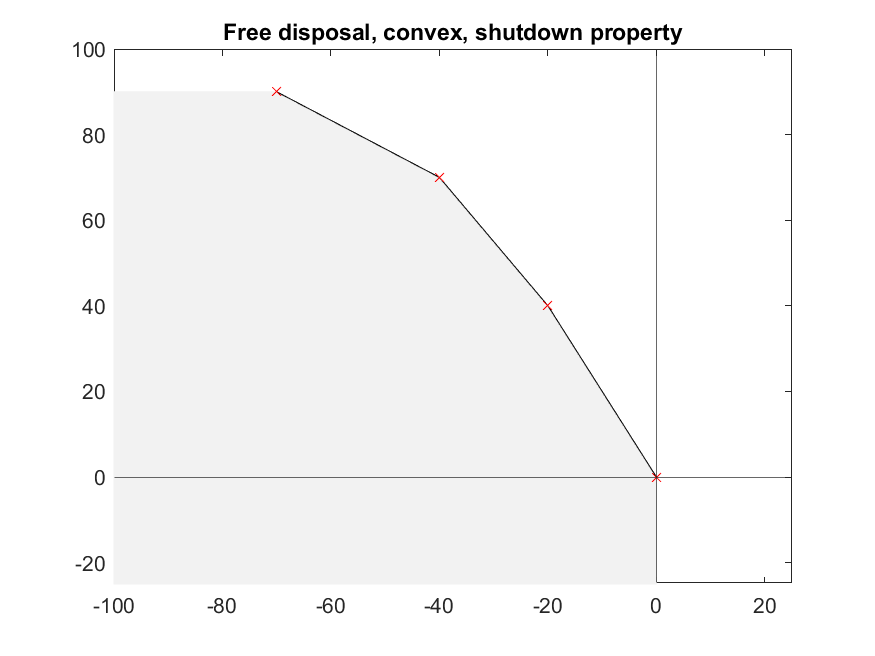
\includegraphics{freedispshutdown}

The above chart shows the realized datapoints, along with the shutdown production option of producing $(0,0)$. It also shows the lines connecting the points, which must be in the set as the set is specified to be convex. The shaded area in the chart show regions attainable by producing at one of the realized levels, not producing, or producing along the lines connecting the realized points, and then utilizing free disposal.

\subsection{Draw the largest production set that can rationalize the data.}
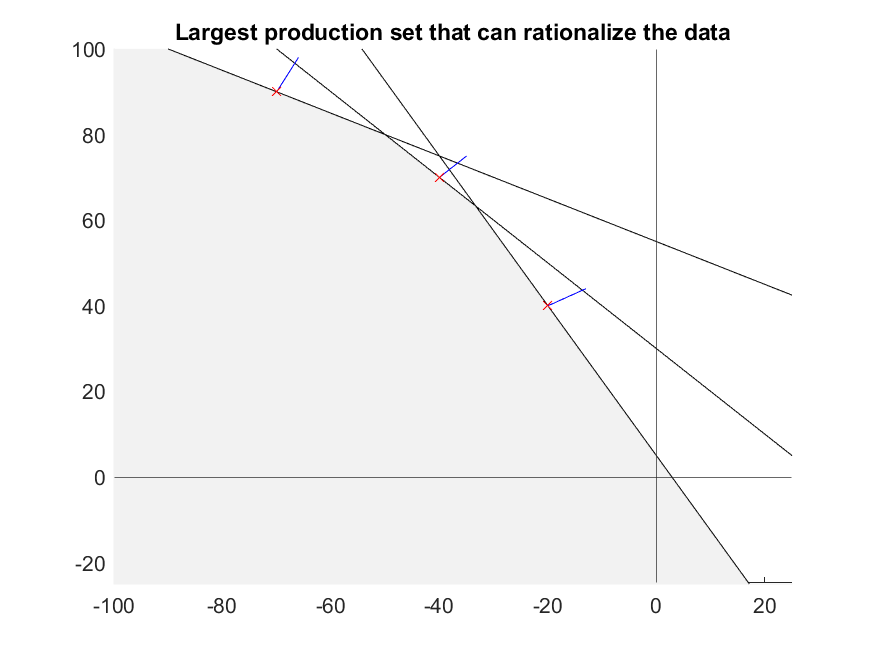
\includegraphics{largestprod}
The above chart shows the realized datapoints (in red), along with (black) lines going through those points that are perpendicular to the price vectors (shown in blue). The shaded region, which includes the lines and the points, represents the largest production set that can rationalize the data.

\section{Question 3}
Define $y(p) = y_1(p) + \dots + y_n(p)$ as the aggregate level of production for the industry at price level $p$, and define $\pi (p) = p \cdot y(p)$. We know that each firm in the industry is profit maximizing and price-taking, and therefore individually each firm satisfies the weak axiom. Thus,
\begin{align*}
\pi (p) &= p \cdot y(p) = p \cdot (y_1(p) + \dots + y_n(p)) = p \cdot y_1(p) + \dots + p \cdot y_n(p) \\ &\geq p \cdot y_1(p^{'}) + \dots + p \cdot y_n(p^{'}) 
= p \cdot (y_1(p^{'}) + \dots y_n(p^{'})) = p \cdot y(p^{'}).
\end{align*}
Therefore, the industry must also satisfy the weak axiom. It can, in a sense of maximizating profit via choosing optimal production vectors, be rationalized as if the industry as a whole was acting as a single profit-maximizing firm. (Note, however, that if the industry as a whole truly was a single firm maximizing profit, then that firm may gain market power and not act as a price-taker. So we should be careful not to take the analogy too far.)

%Let our industry consist of 1 firm. We have then $\pi (p) = p \cdot y(p) = p \cdot y_1(p) \geq  p \cdot y_1p^{'} =  p \cdot y(p^{'})$.
%
%Now, assume that WAPM holds for an industry consisting of n firms. Then we have the following:
%\begin{align*}
%\pi (p) &= p \cdot y(p) = p \cdot (y_1(p) + \dots + y_{n+1}(p)) = p \cdot y_1(p) + \dots + p \cdot y_n(p) + p \cdot y_{n+1}(p) \\ &\geq p \cdot y_1(p^{'}) + \dots + p \cdot y_n(p^{'}) + p \cdot y_{n+1}(p) \geq p \cdot y_1(p^{'}) + \dots + p \cdot y_n(p^{'}) + p \cdot y_{n+1}(p^{'}) \\
%&= p \cdot (y_1(p^{'}) + \dots y_{n+1}(p^{'})) = p \cdot y(p^{'}).
%\end{align*}
%So WAPM holds for an industry consisting of n firms. Thus, by induction, WAPM holds for the industry.
%
%Define $y(p) = \sum\limits_{i \in \mathbb{L}}y_i(p)$ as the aggregate level of production for the industry, where the industry consists of firms in set $\mathbb{L}$, at price level $p$, and define $\pi (p) = p \cdot y(p)$. We know that each firm in the industry is profit maximizing and price-taking, and therefore individually each firm satisfies the weak axiom. Thus,
%\begin{align*}
%\pi (p) &= p \cdot y(p) = p \cdot (\sum_{i \in \mathbb{L}} y_i(p)) = \sum_{i \in \mathbb{L}} p \cdot y_i(p) \\ &\geq  \sum_{i \in \mathbb{L}} p \cdot y_i(p^{'}) 
%= p \cdot ( \sum_{i \in \mathbb{L}}y_i(p^{'}) ) = p \cdot y(p^{'}).
%\end{align*}
%Therefore, the industry must also satisfy the weak axiom. It can, in a sense of maximizating profit via choosing optimal production vectors, be rationalized as if the industry as a whole was acting as a single profit-maximizing firm.
\end{document}
